\documentclass[11pt]{article}
\usepackage{acl2014}
\usepackage{times}
\usepackage{url}
\usepackage{latexsym}
\usepackage{graphicx}
\usepackage{float}

\title{Sentence Generation for Second-Language Learning}

\author{Eugene Koontz\\
  {\tt ekoontz@hiro-tan.org} }

\date{}

\begin{document}
\maketitle
\begin{abstract}
  An implemented web app is described that generates sentence pairs in
  order to provide a quiz-type application for language learning.
\end{abstract}

\section{Introduction}

This is a web application that teaches Italian to English speakers by
displaying English sentences that must be translated to Italian by the
user. After the user submits a guess, the app returns feedback by
showing the user's guess along with the correct Italian translation,
along with feedback about how the user's response was incorrect, if
the app determines it to be incorrect. A Levenshtein distance
algorithm is used to highlight the parts of the guess that the users
guessed incorrectly, to draw the user's attention to these errors.

\begin{figure}[H]
  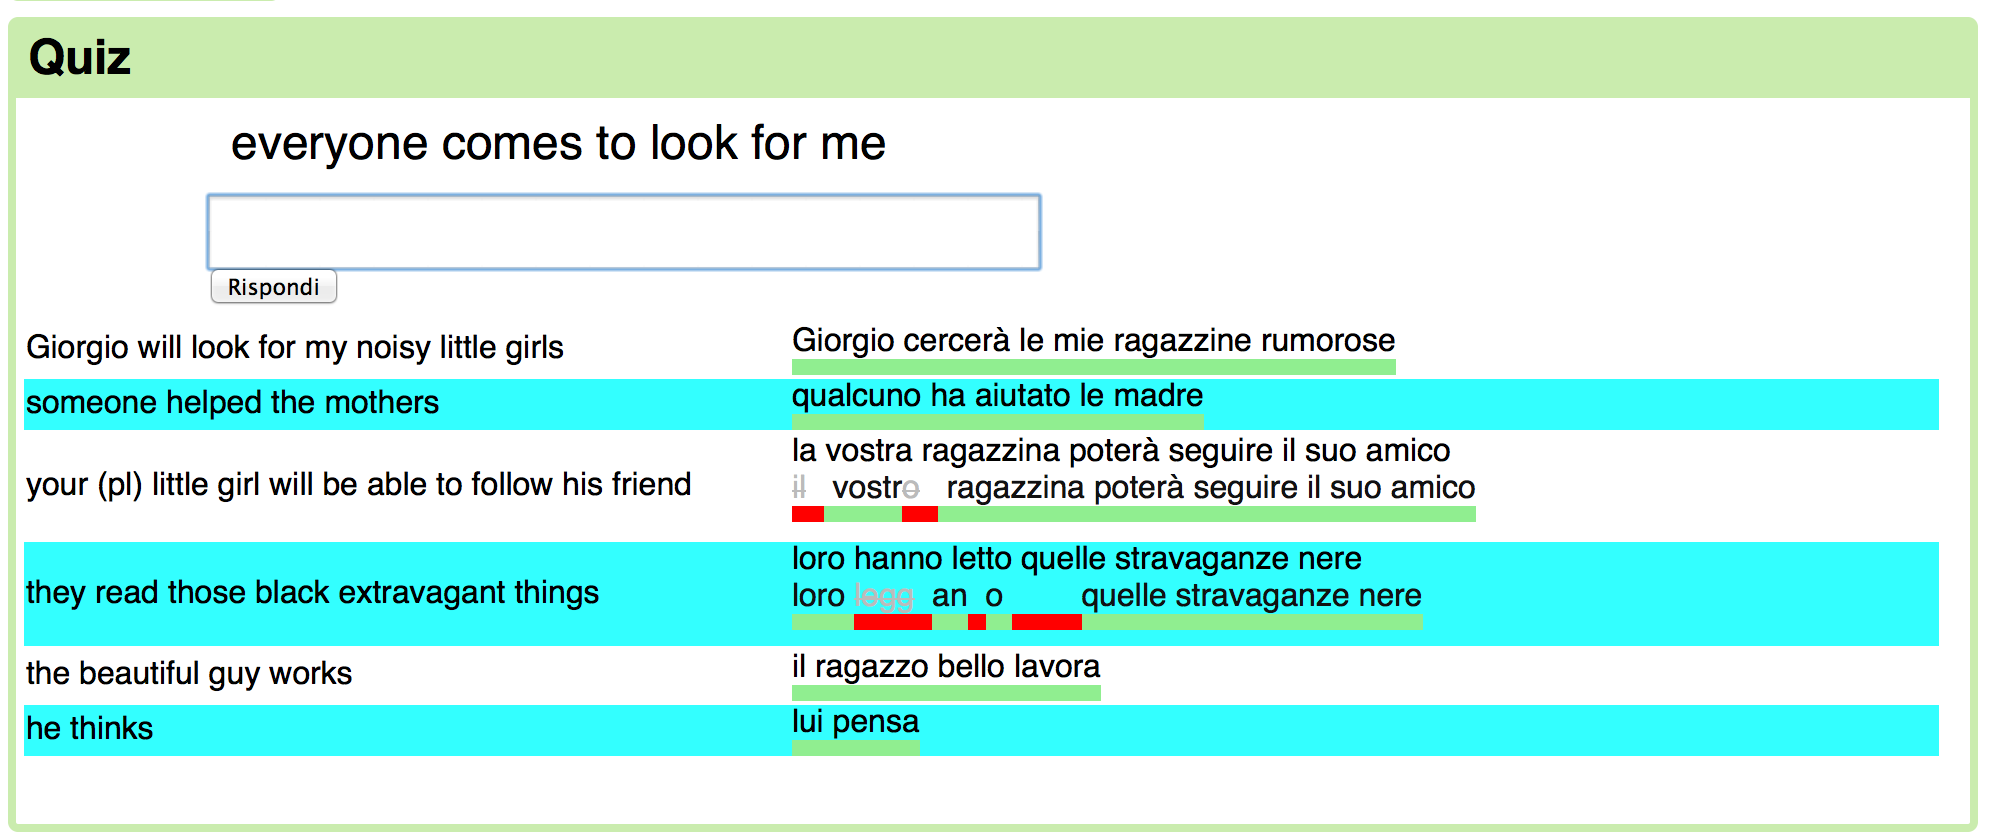
\includegraphics[scale=0.20]{quiz}
  \caption{Quiz UI}
\end{figure}

\section{Background}

The app's linguistic formalism is a straightforward implementation of
HPSG (Head Driven Phrase Structure Grammar) by \cite{PS:94}. In
particular:

\begin{itemize}
\item Linguistic expressions such as words, phrases and sentences are
represented as directed acyclic graphs (DAGs).

\item Structure sharing within such graphs is used to model
  grammatical concepts such as agreement and
  subcategorization. Unification is used combine two or more such
  graphs during parsing or generation.

\item A distinction between phrasal heads and complements - heads select
their complements according to their subcategorization information.

\item Lexemes encode their subcategorization information. This allows
phrase structure rules to be few and fairly abstract, because the
lexemes carry most linguistic information.
\end{itemize}

\section{Sentence Generation}

As explained in the Introduction, the app shows an English sentence to
the user and waits for a guess from the user of an Italian
translation. Behind the scenes, the app has already translated the
expression to Italian. When the user submits a guess, the app compares
this guess with its own translation, and to help the user improve,
highlights the diffrerence between the two translations. 

The sentences are generated by a head-driven, depth first process as
follows.

A grammar $G$ is a set of phrase structure rules.

A sentence specification is a map of features and values that
constrain the generation process. For example a specification of:

\begin{verbatim}
{synsem {sem {subj {human true}}}}
\end{verbatim}

contrains generation to create a phrase whose subject is human.

Given the above definitions, the generator is a function that takes
the grammar, the lexicon, a current depth $d$, and a sentence
specification. 

Given these inputs, the generator:

1. Determines the subset $S$ of the grammar $G$ that is possible given
the specification and the depth. If the depth $d$ is above a specified
constant, the generator returns an empty list.

2. Shuffle the subset $S$. 

3. For each $R \in S$, shuffle the following list:

\begin{itemize}
\item lexical head, lexical complement
\item lexical head, phrasal complement
\item phrasal head, phrasal complement
\item phrasal head, lexical complement
\end{itemize}

4. For each element in this list, if the head is lexical, choose a
lexeme from the lexicon that can be the head of rule $R$. Otherwise,
if the head is phrasal, recursively call the generator, with the depth
$d$ incremented by one. Similarly, if the complement is lexical,
select all lexemes that can be a complement of $R$, and if it is
phrasal, recursively call the generator with a depth reset to zero.

A bounded depth is used to keep the algorithm from decending
endlessly. As described above, the generator will eventually generate all
possible sentences with a given grammar, lexicon, and maximum
depth. In practice however, the generator runs lazily, so that only
the first sentence (chosen randomly) will be generated.

\section{Interactive Development Environment}

Phrases structures can be displayed in HTML as in this figure.

A graphical REPL (Read Evaluate Print Loop) UI allows evaluation of
expressions within a graphical UI that displays phrase structure
trees. Shown here is the response of the system to the user's expression ``np''.
Using this interface, the user can test generation in order to debug
and enhance the grammar and lexicon.

\begin{figure}[H]
  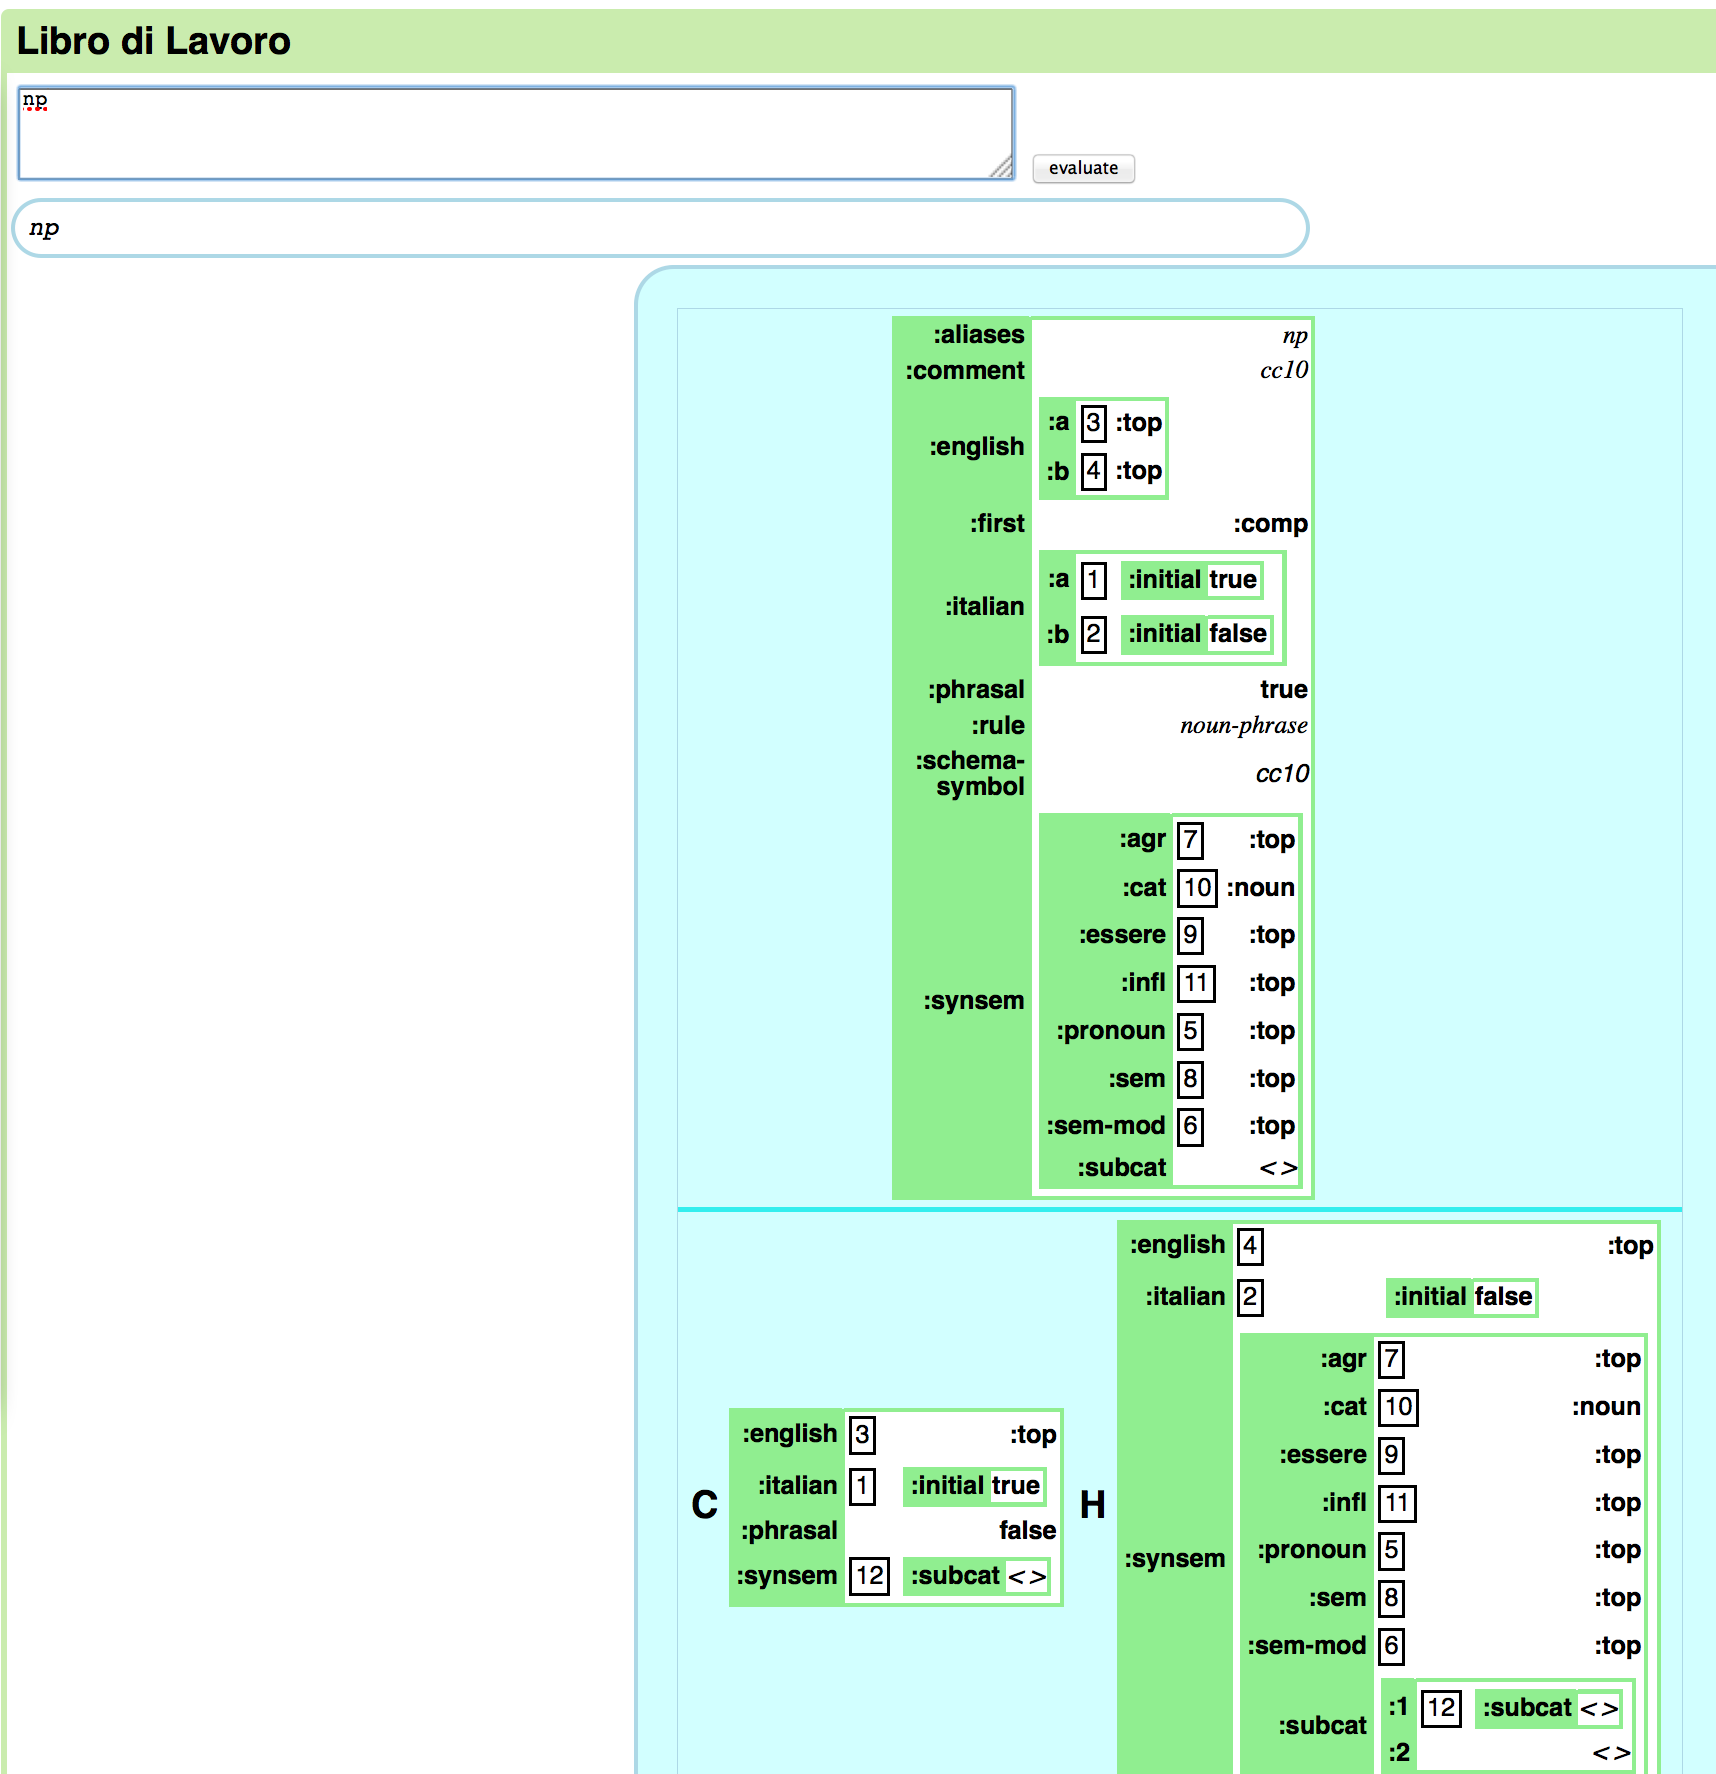
\includegraphics[scale=0.20]{np}
  \caption{Interactive Development Environment}
\end{figure}

\section{Building a user's profile}

A user's errors can be used to guide app to match the user's
deficiencies. Because underlyingly, linguistics expressions are
feature-based, the app can build a profile of the user based on what
questions they answered incorrectly. Those path-values which
correlate with a high error rate indicate that the user needs to be
exposed to more of them in order to improve. For example, if a user
makes errors when conjugating the future tense, this can be correlated
with a high error rate for sentences with the path-value:

\begin{verbatim}
   {synsem {sem {tense future}}}
 \end{verbatim}

\section{Generating felicitous sentences}

Generating high-quality sentences randomly requires care due to
semantic and cultural factors. Merely syntactic correctness is
insufficient: the app must avoid generating sentences like:

``The dog read the book'', or even worse:

``The book read the dog''. 

Constraints preventing either of these are encoded lexically, such as,
 for the verb ``to read'':

\begin{verbatim}
{synsem {sem {pred read
              subj {human true}
                :obj {legible true}}}}
\end{verbatim}

In addition, when the lexicon is loaded, inference rules are applied
to enrich the lexicon with additional information that is implicit -
for example, the lexicon may specify only that ``professor'' is human,
and an inference rule $$ human \rightarrow animate $$ adds the
additional information that a professor is animate also.

\section{Source Code and Demo Site}

Source code is available at:

http://github.com/ekoontz/italianquiz

and is freely available to use under the terms of the GNU Public
License.

A demo site is here: http://hiro-tan.org/italian/

\begin{thebibliography}{}

\bibitem[\protect\citename{Pollard and Sag}1994]{PS:94}
Carl Pollard Ivan Sag.
\newblock 1994.
\newblock {\em Head-Driven Phrase Structure Grammar}.
\newblock CSLI Publications, Stanford, CA.
\end{thebibliography}

\end{document}









